%----------------------------------------------------------------------------------------
%	PACKAGES AND OTHER DOCUMENT CONFIGURATIONS
%----------------------------------------------------------------------------------------

\documentclass[
12pt,
a4paper,
onecolumn,
portrait
]{article}

%%%%%%%%%%%%%%%%%%%%%%%%%%%%%%%%%%%%%%%%%
% Article Notes
% Structure Specification File
% Version 1.0 (1/10/15)
%
% This file has been downloaded from:
% http://www.LaTeXTemplates.com
%
% Authors:
% Vel (vel@latextemplates.com)
% Christopher Eliot (christopher.eliot@hofstra.edu)
% Anthony Dardis (anthony.dardis@hofstra.edu)
%
% License:
% CC BY-NC-SA 3.0 (http://creativecommons.org/licenses/by-nc-sa/3.0/)
%
%%%%%%%%%%%%%%%%%%%%%%%%%%%%%%%%%%%%%%%%%

%----------------------------------------------------------------------------------------
%	REQUIRED PACKAGES
%----------------------------------------------------------------------------------------

\usepackage[includeheadfoot,columnsep=2cm, left=1in, right=1in, top=.5in, bottom=.5in]{geometry} % Margins

%\usepackage[T1]{fontenc} % For international characters
\usepackage[utf8]{inputenc}
%\usepackage{XCharter} % XCharter as the main font

\usepackage{natbib} % Use natbib to manage the reference
%\usepackage{cite}
%\bibliographystyle{apalike} % Citation style
%\bibliographystyle{te} % Citation style

\usepackage[english]{babel} % Use english by default
\usepackage{amsmath}
\usepackage{amssymb}
\usepackage{amsthm}
\usepackage{xcolor}
\usepackage{graphicx}
\usepackage{enumerate}
\usepackage{todonotes}

\newtheorem{df}{Definition}
\newtheorem{ex}{Example}
\newtheorem{as}{Assumption}
\newtheorem{rem}{Remark}
\newtheorem{pr}{Proposition}
\newtheorem{qu}{Question}
\newtheorem{lm}{Lemma}

%----------------------------------------------------------------------------------------
%	CUSTOM COMMANDS
%----------------------------------------------------------------------------------------

\newcommand{\articletitle}[1]{\renewcommand{\articletitle}{#1}} % Define a command for storing the article title
%\newcommand{\articlecitation}[1]{\renewcommand{\articlecitation}{#1}} % Define a command for storing the article citation
\newcommand{\doctitle}{``\articletitle''} % Define a command to store the article information as it will appear in the title and header

\newcommand{\datenotesstarted}[1]{\renewcommand{\datenotesstarted}{#1}} % Define a command to store the date when notes were first made
\newcommand{\docdate}[1]{\renewcommand{\docdate}{#1}} % Define a command to store the date line in the title

\newcommand{\docauthor}[1]{\renewcommand{\docauthor}{#1}} % Define a command for storing the article notes author

% Define a command for the structure of the document title
\newcommand{\printtitle}{
\begin{center}
\textbf{\Large{\doctitle}}

\docdate

\docauthor
\end{center}
}

% set interior
\newcommand{\interior}[1]{%
  {\kern0pt#1}^{\mathrm{o}}%
}

%----------------------------------------------------------------------------------------
%	STRUCTURE MODIFICATIONS
%----------------------------------------------------------------------------------------

\setlength{\parskip}{3pt} % Slightly increase spacing between paragraphs

% Uncomment to center section titles
%\usepackage{sectsty}
%\sectionfont{\centering}

% Uncomment for Roman numerals for section numbers
%\renewcommand\thesection{\Roman{section}}


%----------------------------------------------------------------------------------------
%	ARTICLE INFORMATION
%----------------------------------------------------------------------------------------

\articletitle{Notes on our common PDE model} % The title of the article
\datenotesstarted{October 17, 2016} % The date when these notes were first made
\docdate{\datenotesstarted; rev. \today} % The date when the notes were lasted updated (automatically the current date)

\docauthor{Julian Andrej, Luca Mechelli, \underline{Simon Pirkelmann}} % Your name

%----------------------------------------------------------------------------------------

\begin{document}

\pagestyle{myheadings} % Use custom headers
\markright{\doctitle} % Place the article information into the header

%----------------------------------------------------------------------------------------
%	PRINT ARTICLE INFORMATION
%----------------------------------------------------------------------------------------

\thispagestyle{plain} % Plain formatting on the first page

\printtitle % Print the title

%----------------------------------------------------------------------------------------
%	ARTICLE NOTES
%----------------------------------------------------------------------------------------
\section{Model}
\subsection{Model equations}
I propose we use the following simulation model:
\begin{align}
\frac{\partial \mathbf{y}_1}{\partial t} + \mathbf{y}_1 \cdot \nabla \mathbf{y}_1 &= - \frac{1}{\rho} \nabla y_2 + \nu \Delta \mathbf{y}_1 - \textbf{g} \alpha \Delta y_3 \label{eq:pde-navier-stokes}\\
\nabla \cdot \mathbf{y}_1 &= 0 \label{eq:pde-continuity}\\
\frac{\partial y_3}{\partial t} + \mathbf{y}_1 \cdot \nabla y_3 &= \kappa \Delta y_3 \label{eq:pde-heat-equation}
\end{align}
\begin{align*}
& \mathbf{y}_1: \Omega \times [0, \infty) \rightarrow \mathbb{R}^{d} \text{ is air velocity}  \\
\text{where}\;\;\; &y_2: \Omega \times [0, \infty) \rightarrow \mathbb{R} \;\; \text{ is pressure} \\
&y_3: \Omega \times [0, \infty) \rightarrow \mathbb{R} \;\; \text{ is temperature}
\end{align*}
and coefficients 
\begin{align*}
\rho &: \text{ density of the fluid } \\
\nu  &: \text{ kinematic viscosity } \\
\alpha &: \text{ coefficient of expansion } \\
\kappa &: \text{ thermal diffusivity. } \\
\end{align*}
Some explanation: This model is the so-called Boussinesq approximation of the Navier-Stokes equations, which makes the simplifying assumption that the density of the fluid is constant, which leads to equation \eqref{eq:pde-continuity} (instead of $\frac{\partial \rho}{\partial t} + \nabla \cdot (\rho \mathbf{y}_1) = 0$ in the general form). Equation \eqref{eq:pde-navier-stokes} is the Boussinesq dynamical equation for describing the air flow and equation \eqref{eq:pde-heat-equation} is the equation for the temperature transfer (convection-diffusion). Here the assumption is made that no heat is generated within the domain, i.e. there is no reaction (or source) term.\\
Note that the states $\mathbf{y}_1$ and $y_3$ are directly coupled. This is clear from a physical point of view. A change in temperature ($\Delta y_3$) causes the air to expand or contract which in turn induces an air flow and thus influences the state $\mathbf{y}_1$ (equation \eqref{eq:pde-navier-stokes}). On the other hand the air velocity determines the direction in which the convection term $\nabla y_3$ acts on the temperature in equation \eqref{eq:pde-heat-equation}.

\subsection{Boundary conditions}
Consider the following boundary conditions to the problem
\begin{align}
- \partial_{\nu} \mathbf{y}_1 &= \gamma_1(\mathbf{y}_1 - \mathbf{g}_{D,1}) + \mathbf{g}_{N,1} &\text{ on } &\Gamma \times [0, \infty) \label{eq:pde-boundary-air-velocity-dirichlet} \\
- \partial_{\nu} y_3 &= \gamma_3 (y_3 - g_{D,3}) + g_{N,3} &\text{ on } &\Gamma \times [0, \infty) \label{eq:pde-boundary-heating}\\
\end{align}
where $u_1: \Gamma_1 \times [0, \infty) \rightarrow \mathbb{R}$, $f: \Gamma \times [0, \infty) \rightarrow \mathbb{R}$. \\
This general formulation of the boundary conditions allows for a lot of flexibility in the type of boundary condition we want to consider. \\
For example for the temperature we interpret the function $g_{D,3}$ as the temperature outside of the domain. This means that the flux of the temperature across the boundary is proportional to the difference between the temperatures of the inside and the outside. In this setting the coefficient $\gamma_3$ can be interpreted as the heat permeability of the walls. \\
We can also incorporate the control in this formulation. To control the temperature we might have a radiator on some part of the boundary, which allows us to influence the heat flow into the domain across the boundary. In this case we set the function $g_{N, 3} = u_{3}$ on the part of the boundary where the radiator is located, and $g_{N, 3} = 0$ otherwise.\\
\\
Note that we do not impose boundary conditions on the pressure $y_2$. Instead the pressure should be determined naturally through the model equations.

\subsection{Domain}
For now let's start in 2D and consider the following simple domain:
\begin{align*}
\Omega &= [0, 1] \times [0, 1] \subset \mathbb{R}^{2} \\
\Gamma &= \Omega \setminus \interior{\Omega} \\
\Gamma_1 &= [0, 1] \times \{0\}
\end{align*}
\begin{figure}[h]
\centering
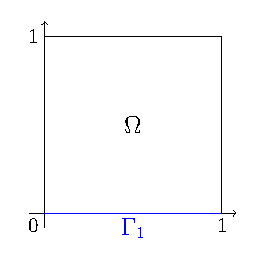
\includegraphics[scale=1.5]{../graphics/domain.pdf}
\caption{Illustration of the domain and the boundary.}
\label{fig:domain-simple}
\end{figure}


\section{Weak form}
TODO!

%----------------------------------------------------------------------------------------
%	BIBLIOGRAPHY
%----------------------------------------------------------------------------------------
\newpage
\renewcommand{\refname}{Reference} % Change the default bibliography title

\nocite{tritton2012physical}

\bibliography{../bibtex} % Input your bibliography file
\bibliographystyle{plain}


%----------------------------------------------------------------------------------------

\end{document}
